\documentclass[a4paper, 11pt]{article}
\usepackage{comment}
\usepackage{fullpage}
\usepackage{amsmath}
\usepackage{amssymb}
\usepackage{mathtools}
\usepackage{fontspec}
\defaultfontfeatures{Ligatures=TeX}
\usepackage{xfrac}
\usepackage{icomma}
\usepackage[section,below]{placeins}
\usepackage[labelfont=bf,font=small,width=0.9\textwidth]{caption}
\usepackage{subcaption}
\usepackage{graphicx}
\usepackage{grffile}
\usepackage{float}
\floatplacement{figure}{htbp}
\floatplacement{table}{htbp}
\usepackage{booktabs}
\usepackage{hyperref}
\usepackage[ngerman]{babel}
\begin{document}
\noindent
%\centerline{\small{\textsc{Technische Universität Dortmund}}} \\
\large{\textbf{9. Übungsblatt zur Vorlesung \hfill WS 2017/2018 \\
Statistische Methoden der Datenanalyse \hfill Prof. W. Rhode}} \\
Annika Burkowitz, Sebastian Bange, Alexander Harnisch \\
\noindent\makebox[\linewidth]{\rule{\textwidth}{0.4pt}}

\section*{Aufgabe 28}
\subsection*{a) b)}
Die drei Attribute, die die höchste Korrelation zum Zielattribut, also dem
Verkaufspreis, aufweisen sind \textit{OverallQual}, \textit{GrLivArea} und
\textit{GarageCars}. Also die Gesamt Qualität, die Fläche des bewohnbaren
Bereiches im Erdgeschoss und die Anzahl der Autos, die insgesamt in die Garage
bzw.\ die Garagen passen. Die Korrelationen sind als Scatter-Plots zusammen mit
Regressionsgeraden in den Abbildungen~\ref{fig:Scatter_OverallQual}
bis~\ref{fig:Scatter_GarageCars} dargestellt.
\begin{figure}
    \centering
    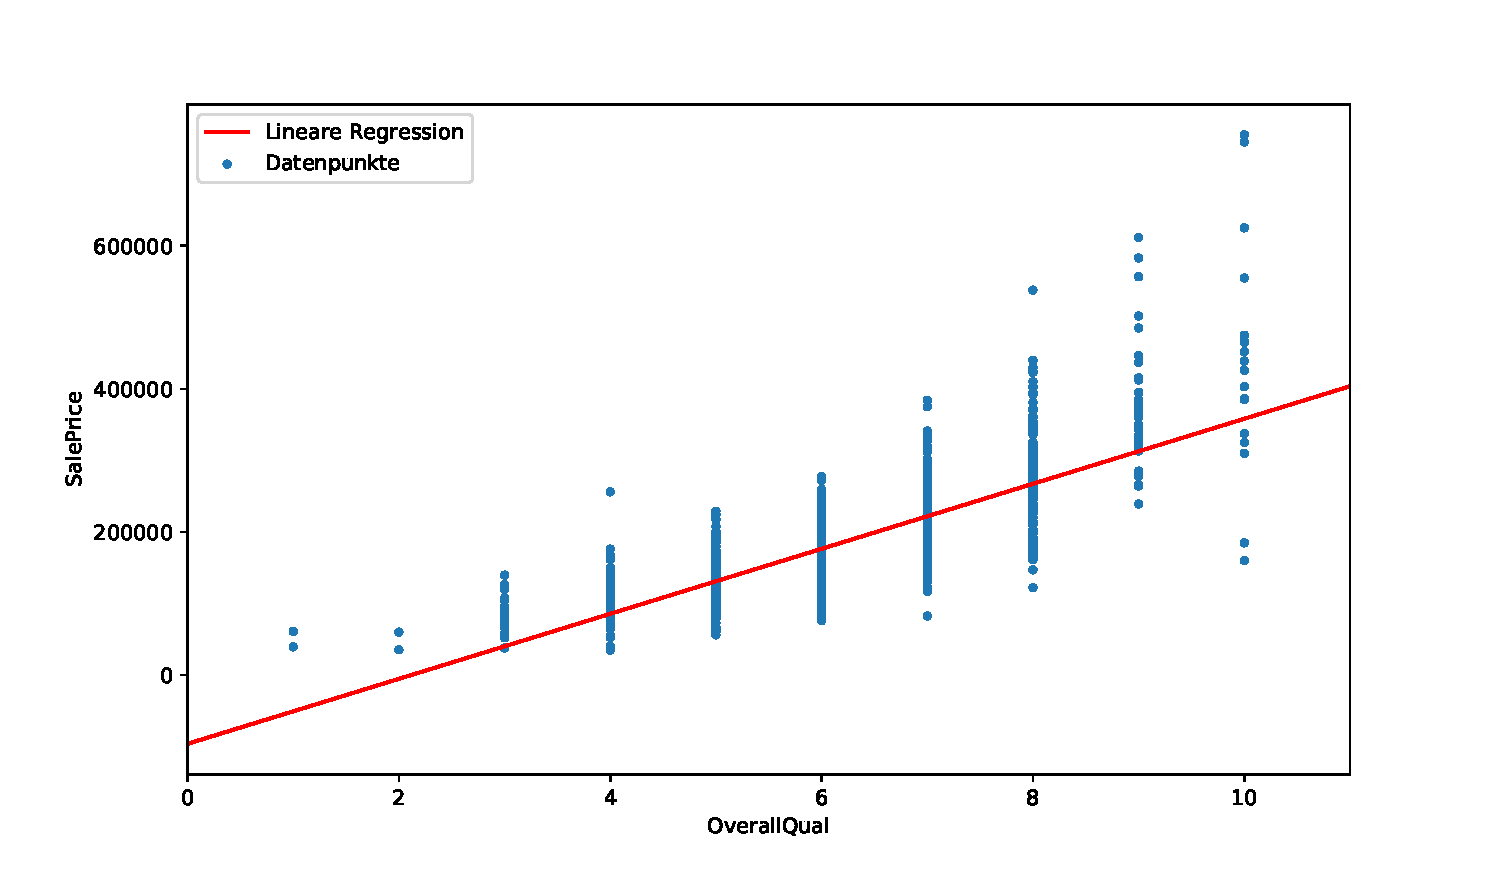
\includegraphics[width=\textwidth]{../A28abc/Scatter_OverallQual.pdf}
    \caption{Korrelation zwischen \textit{OverallQual} und \textit{SalePrice}.}
    \label{fig:Scatter_OverallQual}
\end{figure}
\begin{figure}
    \centering
    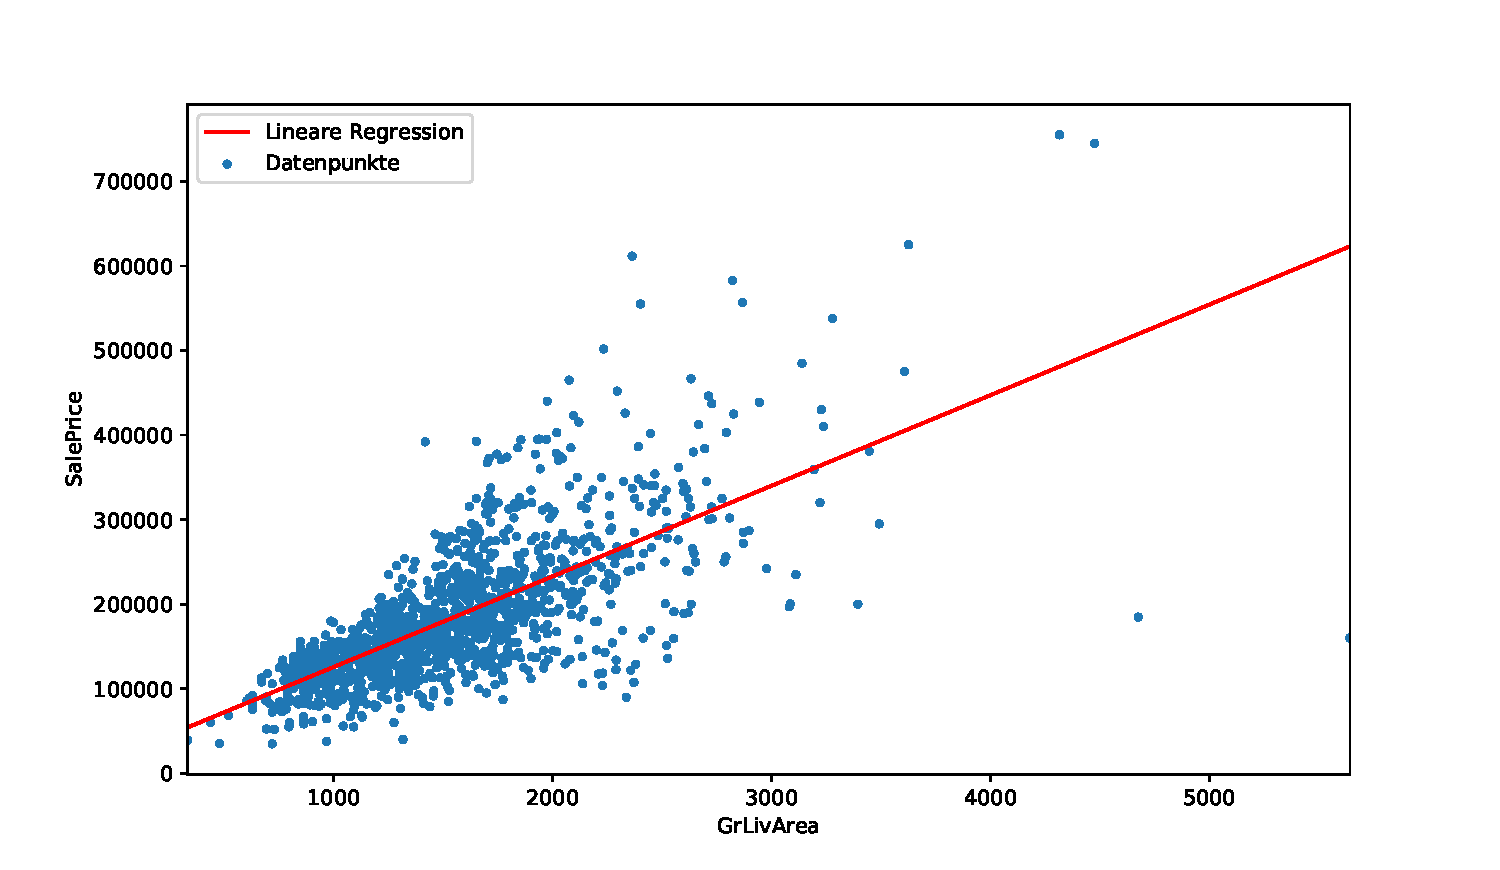
\includegraphics[width=\textwidth]{../A28abc/Scatter_GrLivArea.pdf}
    \caption{Korrelation zwischen \textit{GrLivArea} und \textit{SalePrice}.}
    \label{fig:Scatter_GrLivArea}
\end{figure}
\begin{figure}
    \centering
    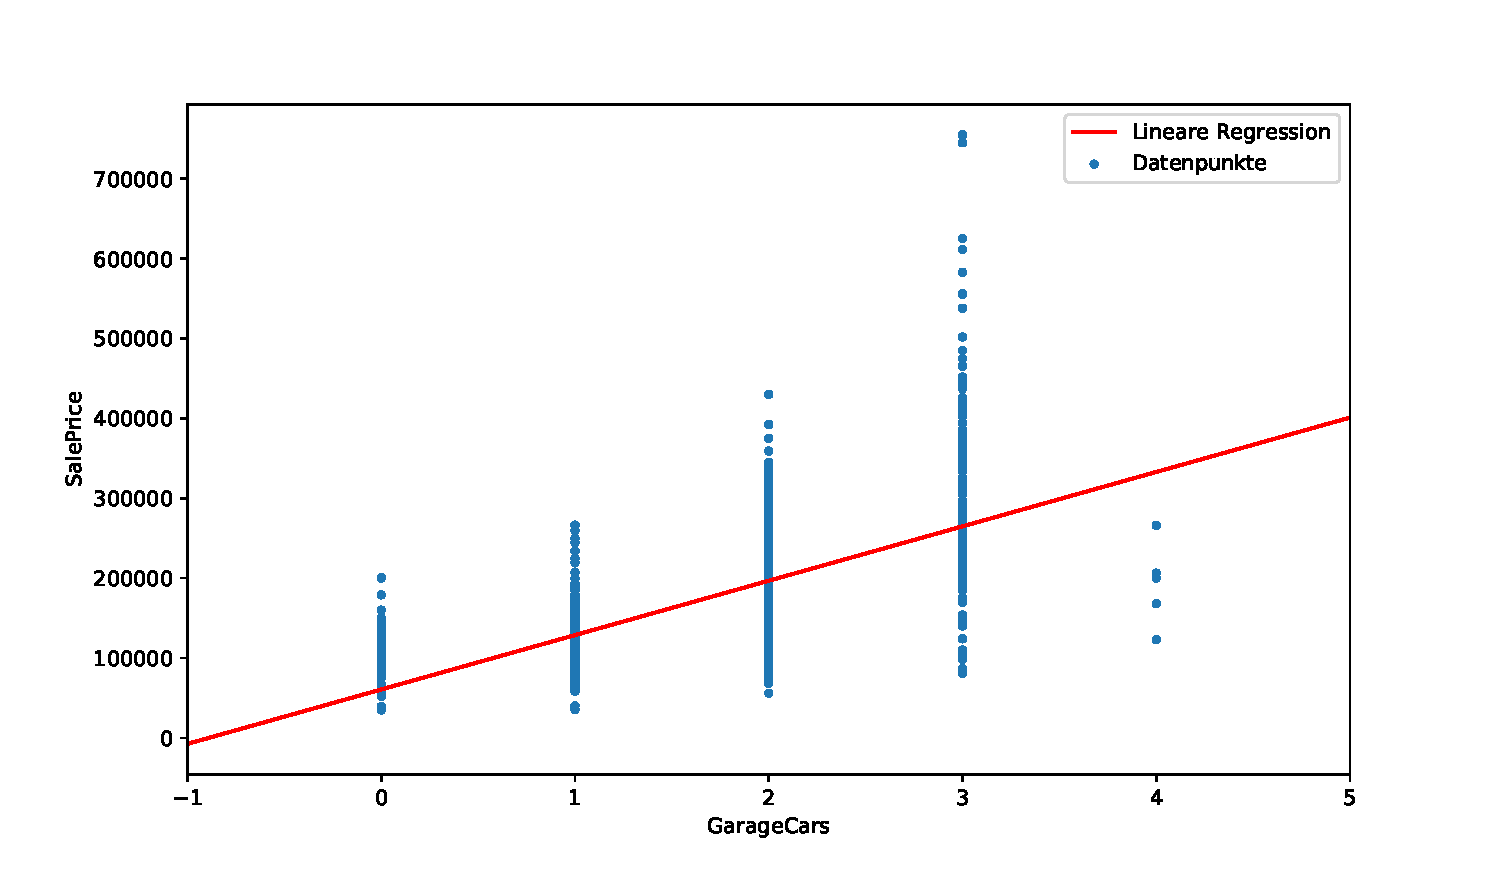
\includegraphics[width=\textwidth]{../A28abc/Scatter_GarageCars.pdf}
    \caption{Korrelation zwischen \textit{GarageCars} und \textit{SalePrice}.}
    \label{fig:Scatter_GarageCars}
\end{figure}
\FloatBarrier

\subsection{c)}
Die relativen Abstände zwischen den geschätzten Verkaufspreisen aus den
linearen Regressionen und den wahren Verkaufspreisen sind in den
Histogrammen~\ref{fig:Hist_OverallQual} bis~\ref{fig:Hist_GarageCars}
dargestellt.

\begin{figure}
    \centering
    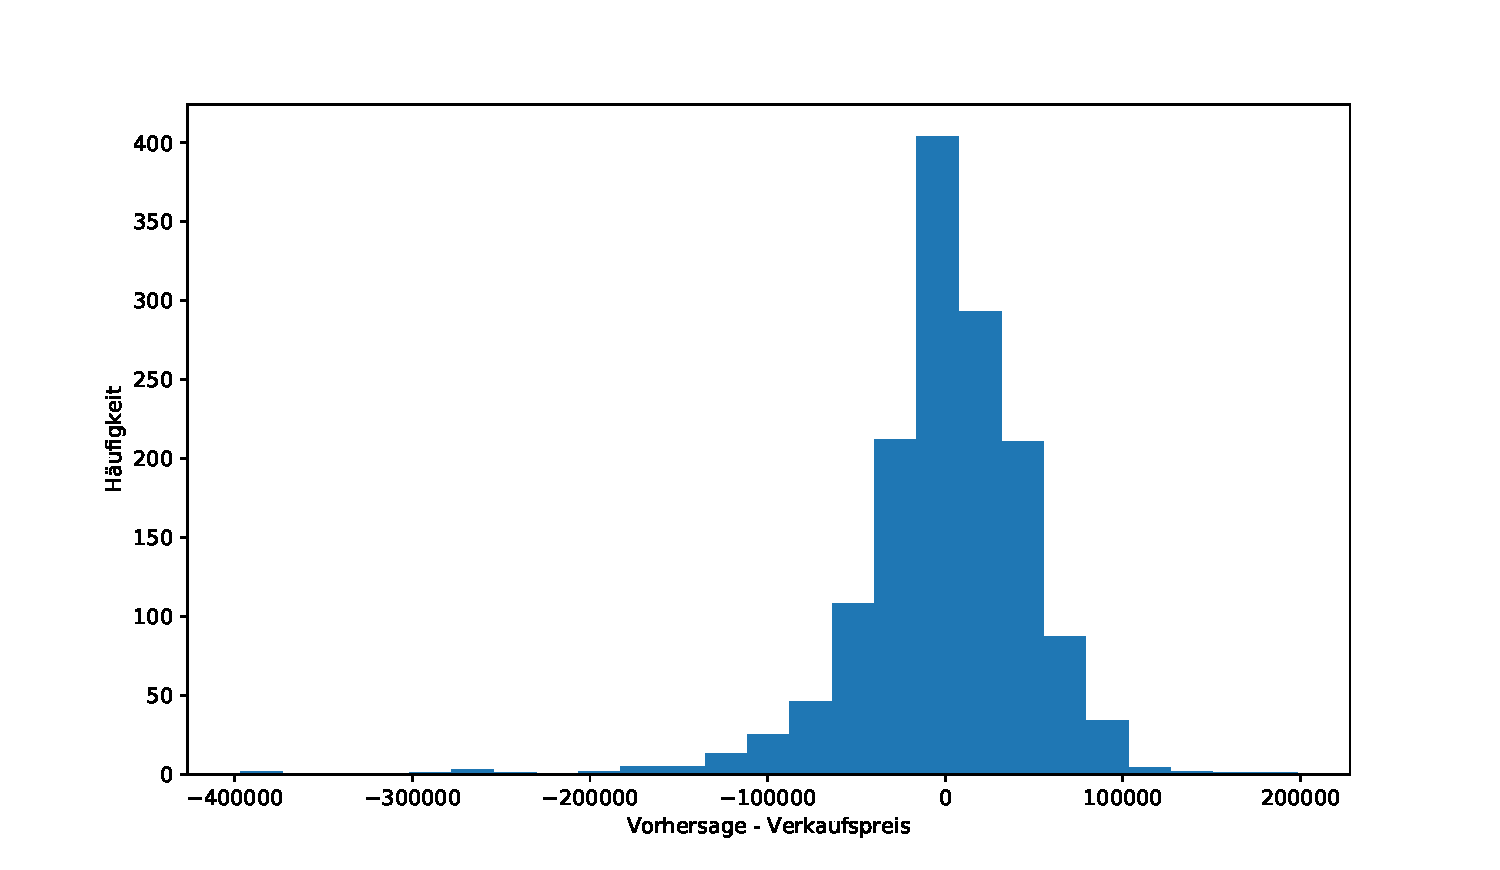
\includegraphics[width=\textwidth]{../A28abc/Hist_OverallQual.pdf}
    \caption{Histogramm der relativen Abstände zwischen dem vorhergesagten und dem tatsächlichen Verkaufspreis für das Attribut \textit{OverallQual}.}
    \label{fig:Hist_OverallQual}
\end{figure}
\begin{figure}
    \centering
    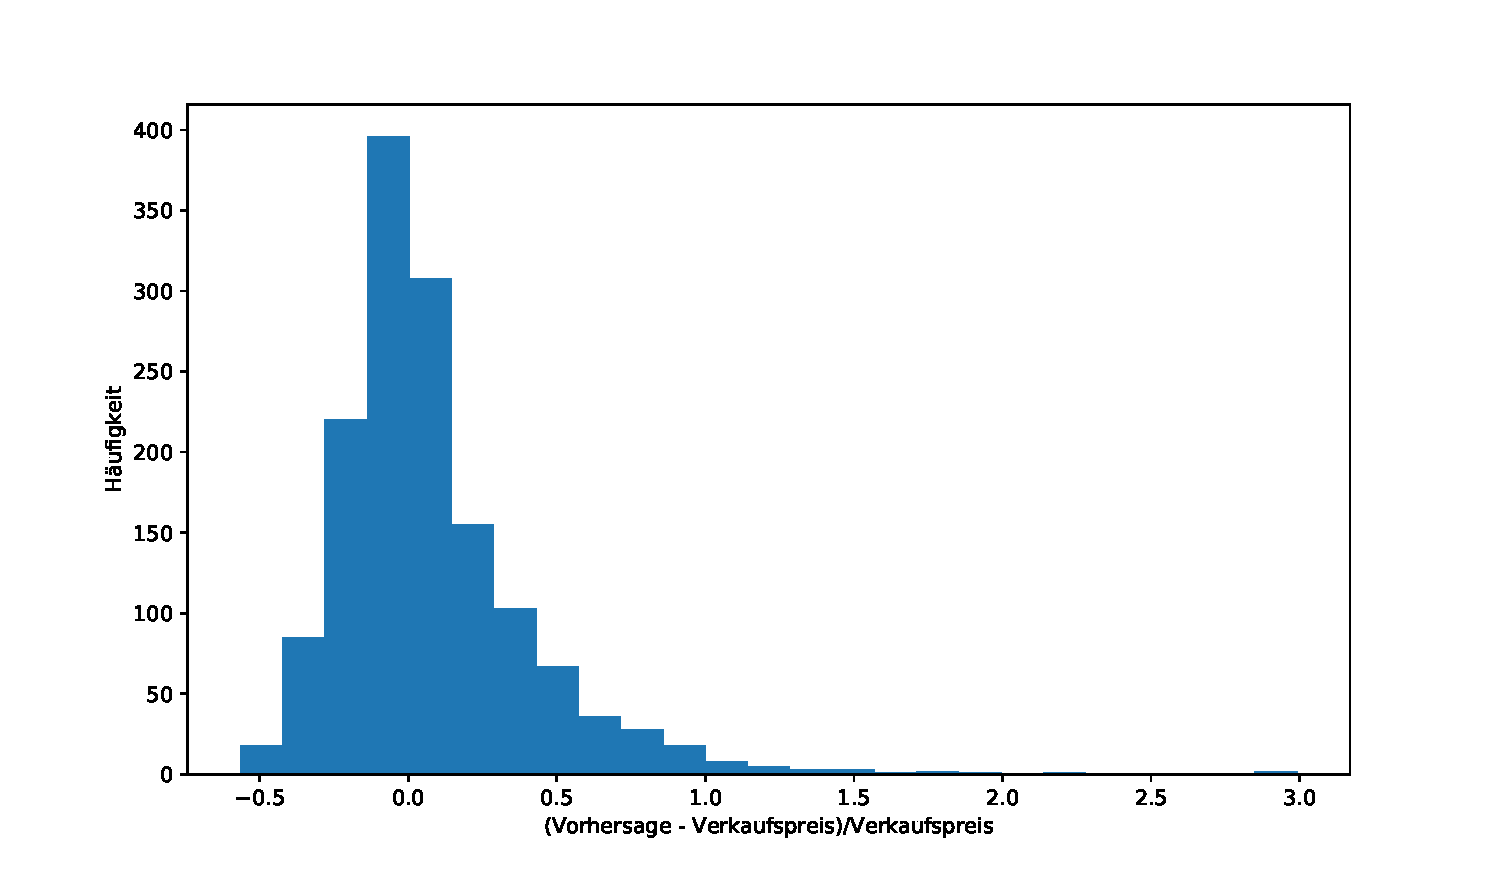
\includegraphics[width=\textwidth]{../A28abc/Hist_GrLivArea.pdf}
    \caption{Histogramm der relativen Abstände zwischen dem vorhergesagten und dem tatsächlichen Verkaufspreis für das Attribut \textit{GrLivArea}.}
    \label{fig:Hist_GrLivArea}
\end{figure}
\begin{figure}
    \centering
    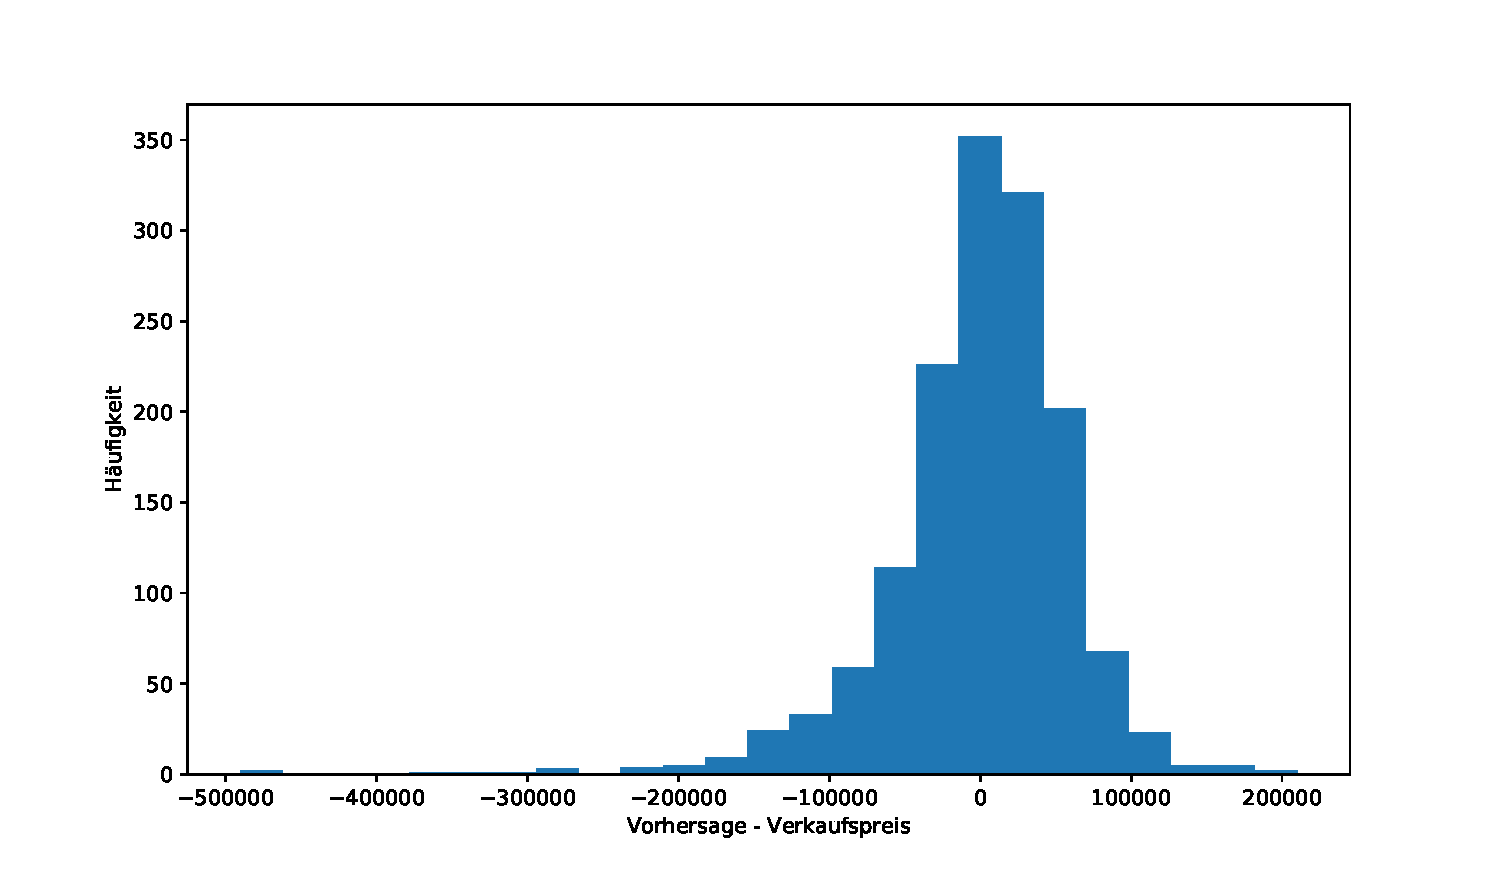
\includegraphics[width=\textwidth]{../A28abc/Hist_GarageCars.pdf}
    \caption{Histogramm der relativen Abstände zwischen dem vorhergesagten und dem tatsächlichen Verkaufspreis für das Attribut \textit{GarageCars}.}
    \label{fig:Hist_GarageCars}
\end{figure}
\FloatBarrier

\section*{Aufgabe 28 d) - Data-Mining Challenge}
Insgesamt hatten wir zu wenig Zeit, um die Challenge zu unserer eigenen Zufriedenheit zu bearbeiten. Darum war die Idee ersteinmal von Kernels auf Kaggle zu lernen und als Basis damit selbst zu versuchen weiterzumachen. Leider haben wir es nicht geschafft, den Score des Kernels~\cite{kernel} zu verbessern. Unser bester public Score von $0,11968$ ist der mit XGBoost~\cite{xgboost} ohne Änderungen aus~\cite{kernel}, daher keine Eigenleistung. Wir waren allerdings wirklich interessiert daran, ob wir es schaffen würden mit neuronalen Netzen, die ja nach allgemeiner aktueller Meinung für tabellarische Probleme eher weniger geeignet sind, als geboostete Entscheidungsbäume, diesen Score zu übertreffen oder zumindest ähnlich gute Ergebnisse zu erzielen. Übertreffen konnten wir ihn leider nicht, allerdings sind wir zumindest nach unserer eigenen Crossvalidation auf den Trainingsdaten zu ähnlich guten Ergebnissen gekommen. Der beste public Score viel allerdings mit $0,13084$ schlechter aus, als unser CV-Score. Mit einem neuronalen Netz ähnliche gute Ergebnisse zu erzielen war jedoch deutlich schwerer und zeitaufwändigerer als anfänglich gedacht. Und auch wenn dies leider trotzdem ein Misserfolg war, wissen wir so nun zumindest, dass Entscheidungsbäume hier wirklich das bessere Verfahren zu sein scheinen. Wir haben es immerhin geschafft, den public Score von neuronalen Netzen durch Anpassen der Architektur und Featureselection von $0,20233$ (minimalistisches neuronales Netz ohne Featureselection) auf $0,13092$ (komplexere Architektur und Featureselection) zu verbessern. Unser bestes Ergebnis von $0,13084$ nach dem Publicscore hat jedoch das selbe Netz ohne Featureselection erzielt, was unserer Meinung nach aber einfach nur unglücklicher Zufall sein sollte, da unser Netz mit Featureselection in CV auf den Trainingsdaten etwas besser abgeschnitten hat, als ohne Featureselection.

Wir haben es nicht geschafft durch eigenes Feature Engineering irgendetwas gegenüber~\cite{kernel} zu verbessern. Trotzdem haben wir natürlich nachvollzogen und verstanden, wobei es beim Feature Engineering auf diesen Daten ankommt. Daher beschreiben wir dies hier auch nochmal. Unsere Eigenleistung hier besteht darin eine relativ gute Netzarchitektur zu finden und für diese Architektur eine Featureselection durchzuführen, auch wenn man hier mit mehr Zeit sicherlich noch sehr viel mehr rausholen könnte.

Das endgültige Ergebnis sollte mit unserem Code replizierbar sein, die Optimierung des Modells und der Featureselection allerdings nicht, da viel von dem dafür verwendeten Code nicht mehr in der exakt auszuführenden Form übrig ist, da er relativ unsauber dauernd manuell angepasst wurde. Um hier streng sauber wissenschaftlich zu arbeiten fehlte die Zeit. Außerdem haben wir allein für die Featureselection insgesamt etwa 10 Stunden Rechenzeit auf einer GeForce GTX 1060 investiert.

Die Kommentare in der Abgabe sind auf Englisch, um konsistent zu sein und den Code eventuell online teilen zu können.

\subsection*{Vorbereiten der Daten und Feature Engineering}
Das in der Abgabe stehende Feature Engineering stammt in dieser Form nicht von uns, sondern von~\cite{kernel}. Eigentlich sollte alles durch die Kommentare, die auch von von~\cite{kernel} stammen, erklärt sein. Aus den ursprünglich 81 Features werden insgesamt 407 Features generiert. Hier nochmal kurz das Wichtigste:
\begin{itemize}
    \item Aussortieren von Ausreißern
    \item Fehlende Werte ersetzen, beispielsweise durch Median (LotFrontage)
    \item One-Hot Encoding von kategorischen Features
    \item Logarithmieren der Verkaufspreise, da diese lognormal verteilt sind
    \item Qualitätsbewertungen von Wörtern in Zahlen konvertieren
    \item Vereinfachungen durchführen. Beispielsweise sind die Meisten Grundstücke eben, daher LandContour ein binäres Feature IsLevel generieren. Oder auch das Zusammenfassen der Nachbarschaften in Bins.
    \item Kreatives hinzufügen von eigenen Features. Das ist wohl der schwierigste und zeitaufwändigste Teil. Beispielsweise ein Feature, das die Hochsaison der Verkäufe beschreibt
\end{itemize}

\subsection*{Netzarchitektur}
Wir verwenden Keras~\cite{keras} mit Tensorflow~\cite{tf} als Backend. Tensorflow wurde unter Arch Linux mit CUDA Support kompeliert, und wird auf einer GeForce GTX 1060 ausgeführt. Zum Bewerten verschiedener Netze wird 10 fache Crossvalidation auf den Trainingsdaten durchgeführt. Außerdem wird vorher der Trainingsfortschritt auf den gesamten Trainingsdaten mit 20\% Testdatensplit durchgeführt, um grob eine Vorstellung des Lernerfolges zu kriegen und eine geeignete Anzahl an Epochs für die Crossvalidation zu wählen.

Die größten Verbesserungen konnten durch Batchnormalization und Dropout nach jedem Layer erzielt werden. Entgegen der allgemein vorherrschenden Empfehlung sind die Ergebnisse jedoch viel besser, wenn immer nach der Aktivierung normalisiert wird, und nicht davor. Die Batchsize wurde als Hyperparameter optimiert und mit 200 relativ groß gewählt. Dafür muss natürlich über mehr Epochs trainiert werden.

Regularisierung durch Dropout mit einer Rate von $0,2$ hat das Lernen deutlich geglättet und verhindert erfolgreich Overfitting\footnote{Tut mir Leid, aber ich hab jetzt leider zu wenig Zeit um für all das Plotts zu erstellen\dots}.

Letztlich besteht die verwendete Architektur aus drei fully connected Layern, die so viele Neuronen haben wie es Features gibt. Darauf folgen, je nach Anzahl der Features, vier bis sechs fully connected Layers, deren Neuronenzahl sich von Layer zu Layer halbiert, wobei es zwei Layer mit 50 Neuronen gibt. Es wird für alle Layer relu als Aktivierungsfunktion verwendet, kurze Experimente mit leaky relu haben zu deutlichen Verschlechterungen geführt.

Als Benchmark wurde ein minimalistisches Netz verwendet, das nur einen fully connected hidden Layer mit so vielen Neurononen wie Inputs hat. Die Performance\footnote{Hier angegeben als Ergebnis von 10-facher Crossvalidation.} gegenüber diesem Netz von $0,18 \pm 0,03$ konnte deutlich verbessert werden auf $0,12 \pm 0,02$. Das verwendete Fehlermaß ist die Wurzel aus der mittleren quadrierten Differenz der logarithmierten Verkaufspreise.

\subsection*{Featureselection}
Es werden Entscheidungsbäume (XGBoost~\cite{xgboost}) verwendet, um Scores für die Features zu erstellen. Anschließend wird mittels Crossvalidation für verschiedene Feature Score Thresholds getestet, wie die gewählte Netzarchitektur mit den unterschiedlichen Selektionen abschneidet. Dabei werden immer aus einem manuell gewählten Bereich, der interessant sein könnte, gleichverteilt zufällige Thresholds aus den vorkommenden Scores gezogen. Das Ergebnis ist in Abbildung~\ref{fig:fs} dargestellt.
\begin{figure}
    \centering
    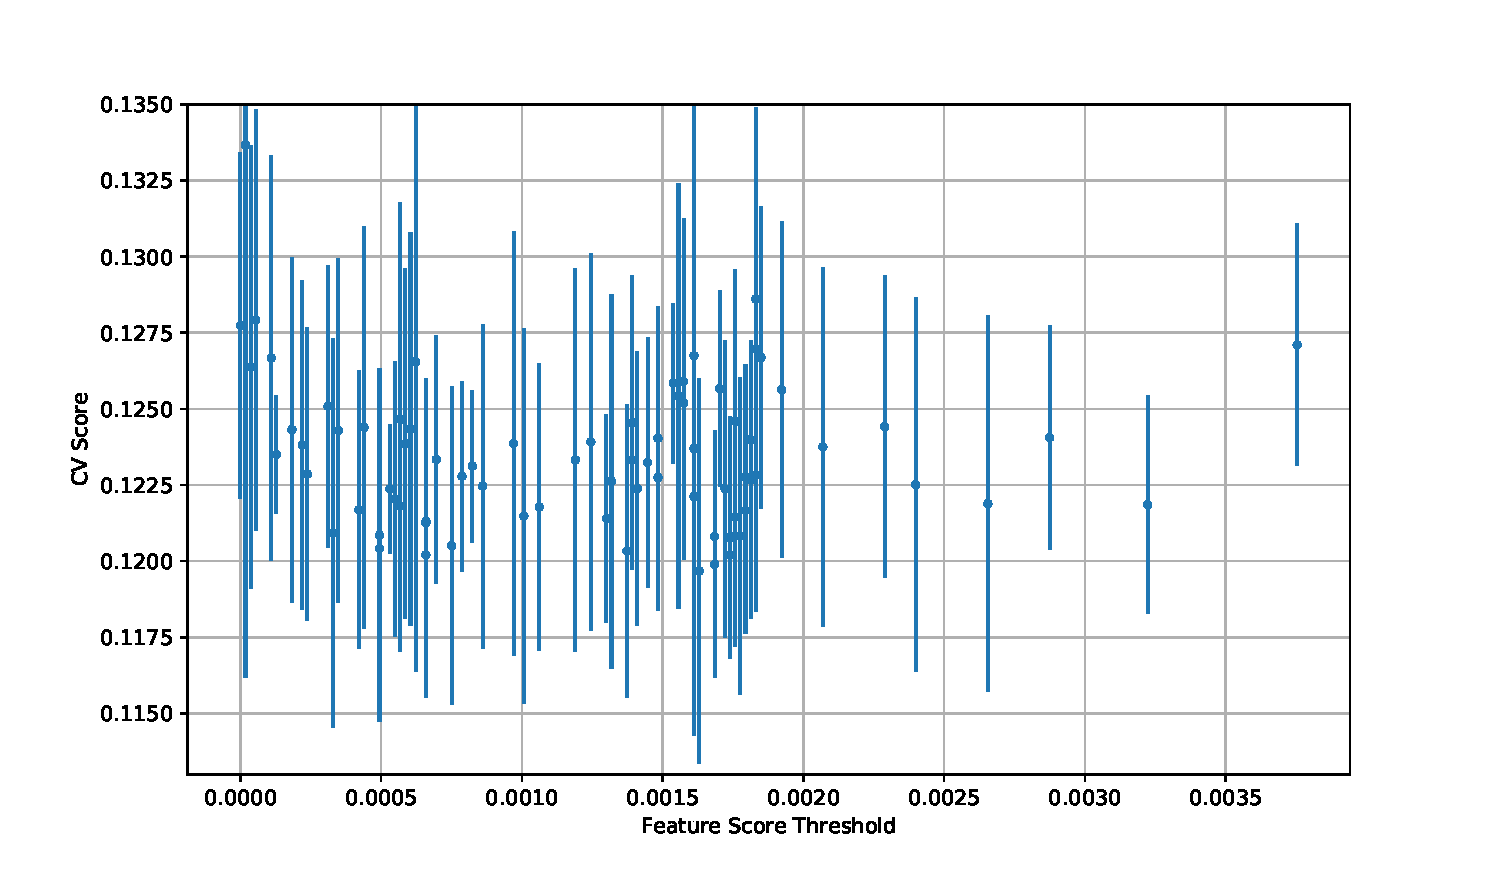
\includegraphics[width=\textwidth]{../Challenge/feature_scores.pdf}
    \caption{Crossvalidation Score für verschiedene Feature Score Thresholds.}
    \label{fig:fs}
\end{figure}

Es ist ein Abwärtstrend für das Aussortieren der schlechtesten Features erkennbar. Insgesamt scheint die Featureselection allerdings keine sehr großen Verbesserungen zu erzielen, es lässt sich allerdings ein Minimum bei 0,0016 erahnen. Wir wählen als Threshold 0,00162974, mit diesem sind noch 156 der 407 Features übrig, was zumindest den Vorteil hat, dass das Training so sehr viel weniger aufwändig ist, was in der Praxis allerdings nur bedingt relevant ist.

Die gewählte Vorgehensweise ist kritisch zu sehen, da in der Featureselection bereits Information aus den gesamten Trainingsdaten enthalten ist, und nicht nur aus denen, die in den jeweiligen Splitts der Crossvalidation zum Training verwendet werden. Streng genommen müsste die Featureselection für jedne Crossvalidation Split neu durchgeführt werden um ein wirklich absolut sauberes Ergebnis zu erhalten.

\subsection*{Ergebnisse}
Wenn ihr wirklich nur nach dem Publicscore gehen wollt, dann beinhaltet \textit{submission\_xgb.csv} unser bestes Ergebnis von 0,11968, das allein beinhaltet aber praktisch keine Eigenleistung. Unser Ergebnis mit neuronalem Netz und Featureselection aus \textit{submission\_0.csv} ist mit 0,13092 deutlich schlechter und fällt sogar etwas schlechter aus als der Score von 0,13084 ohne Featureselection, was jedoch einfach Zufall sein sollte. Nach unserer Crossvalidation sind die Ergebnisse mit Featureselection etwas besser, als ohne Featureselection. Also letzlich haben wir auf Grund von Zeitmangel eigentlich nur einen Vergleich zwischen XGBoost und neuronalen Netzen durchgeführt und gezeigt, dass man durchaus neuronale Netze verwenden kann, XGBoost mit einem CV Score von $0,11 \pm 0,01$ auf den selben 10 Splitts jedoch in diesem Fall wirklich besser ist.

\begin{thebibliography}{9}
    \bibitem{kernel}
    Human Analog
    \textit{XGBoost + Lasso - Kaggle Kernel}
    \url{https://www.kaggle.com/humananalog/xgboost-lasso/}

    \bibitem{xgboost}
    \textit{XGBoost}
    \url{https://github.com/dmlc/xgboost/tree/master/python-package}

    \bibitem{keras}
    \textit{Keras}
    \url{https://github.com/keras-team/keras}

    \bibitem{tf}
    Google
    \textit{Tensorflow}
    \url{https://www.tensorflow.org}
\end{thebibliography}
\end{document}
